

\tikzset{every picture/.style={line width=0.75pt}} %set default line width to 0.75pt        

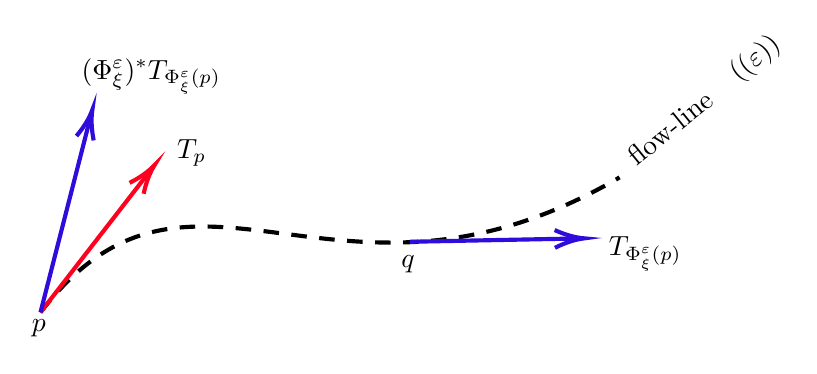
\begin{tikzpicture}[x=0.75pt,y=0.75pt,yscale=-1,xscale=1]
%uncomment if require: \path (0,300); %set diagram left start at 0, and has height of 300

%Curve Lines [id:da8863758369081609] 
\draw [line width=1.5]  [dash pattern={on 5.63pt off 4.5pt}]  (145.68,192.32) .. controls (218.68,97.32) and (287.68,207.32) .. (424.68,127.32) ;
%Straight Lines [id:da25242491594252703] 
\draw [color={rgb, 255:red, 255; green, 0; blue, 31 }  ,draw opacity=1 ][line width=1.5]    (145.68,192.32) -- (198.85,123.69) ;
\draw [shift={(200.68,121.32)}, rotate = 127.76] [color={rgb, 255:red, 255; green, 0; blue, 31 }  ,draw opacity=1 ][line width=1.5]    (14.21,-4.28) .. controls (9.04,-1.82) and (4.3,-0.39) .. (0,0) .. controls (4.3,0.39) and (9.04,1.82) .. (14.21,4.28)   ;
%Straight Lines [id:da3778353955646855] 
\draw [color={rgb, 255:red, 47; green, 11; blue, 220 }  ,draw opacity=1 ][line width=1.5]    (323.68,158.32) -- (404.68,156.73) ;
\draw [shift={(407.68,156.67)}, rotate = 178.87] [color={rgb, 255:red, 47; green, 11; blue, 220 }  ,draw opacity=1 ][line width=1.5]    (14.21,-4.28) .. controls (9.04,-1.82) and (4.3,-0.39) .. (0,0) .. controls (4.3,0.39) and (9.04,1.82) .. (14.21,4.28)   ;
%Straight Lines [id:da5542891074051847] 
\draw [color={rgb, 255:red, 47; green, 11; blue, 220 }  ,draw opacity=1 ][line width=1.5]    (145.68,192.32) -- (169.94,97.57) ;
\draw [shift={(170.68,94.67)}, rotate = 104.36] [color={rgb, 255:red, 47; green, 11; blue, 220 }  ,draw opacity=1 ][line width=1.5]    (14.21,-4.28) .. controls (9.04,-1.82) and (4.3,-0.39) .. (0,0) .. controls (4.3,0.39) and (9.04,1.82) .. (14.21,4.28)   ;

% Text Node
\draw (140,194.4) node [anchor=north west][inner sep=0.75pt]    {$p$};
% Text Node
\draw (318,163.4) node [anchor=north west][inner sep=0.75pt]    {$q$};
% Text Node
\draw (210,107.4) node [anchor=north west][inner sep=0.75pt]    {$T_{p}$};
% Text Node
\draw (418,154.4) node [anchor=north west][inner sep=0.75pt]    {$T_{\boldsymbol{\Phi}^\varepsilon_\xi(p)}$};
% Text Node
\draw (424.99,114.8) node [anchor=north west][inner sep=0.75pt]  [rotate=-321.06] [align=left] {flow-line};
% Text Node
\draw (473.35,73.28) node [anchor=north west][inner sep=0.75pt]  [rotate=-321.1]  {$( \upsigma ( \varepsilon ))$};
% Text Node
\draw (164,68.4) node [anchor=north west][inner sep=0.75pt]    {$\qty(\boldsymbol{\Phi}^\varepsilon_\xi)^* T_{\boldsymbol{\Phi}^\varepsilon_\xi(p)}$};


\end{tikzpicture}
